\documentclass[12pt, reqno]{amsart}
\usepackage{amsmath, amsthm, amscd, amsfonts, amssymb, graphicx, color, tabto}
\usepackage[bookmarksnumbered, colorlinks, plainpages]{hyperref}

\textheight 22.5truecm \textwidth 14.5truecm
\graphicspath{{img/}} %configuring the graphicx package
\setlength{\oddsidemargin}{0.35in}\setlength{\evensidemargin}{0.35in}
\setlength{\topmargin}{-.5cm}
\numberwithin{equation}{section}
\begin{document}
\setcounter{page}{1}



\centerline{}

\centerline{}

\title{Do we even need better page replacement algorithms?}
\subtitle{A contemplation from a efficiency and economically focussed point of view}

\author{Mathis Burger}

\begin{abstract}
Developing new page replacement algorithms is quite expensive and time consuming. But do we even need to research for new ones? Or can we
increase the performance of page replacement though other methods and technics more cost efficient for all? This paper takes some simulations
and checks the dependency of three variables to the amount of page faults.
\end{abstract} \maketitle

\section{Introduction and preliminaries}

\noindent Page replacement algorithms are essential when it comes to improving the performance of the computers memory. Therefore, computer scientists developed many
approaches to come even closer to the ideal algorithm as a benchmark. I have asked myself if it is even economically worth it to develop new algorithms. We are able to increase the
size of the memory over the efficiency of PR-algorithms. Is there still a need for new algorithms or will the current algorithms meet our needs in the future of computing?

\section{Simulation conditions}

Through the rise of ubiquitous computing there are many different constellations of hardware configuration.
I took the most common and also took a forefast to possible situations in the future.
\begin{enumerate}
    \item \textbf{Low memory; short reference; low page variety} is a configuration often found in small IOT devices 
    with limited functionality or in smart medical devices with limited functionality.
    \item \textbf{Low memory; long reference; low page variety} as a hardware configuration is often found in cheap IOT devices 
    that are developed to have longer response times, but be cheaper then faster ones.
    \item \textbf{High memory; short reference; low page variety} is mainly used in high response time
    IOT devices or in devices that are designed to execute a certain task very fast.
    \item \textbf{High memory; long reference; low page variety} is often used for standard desktop PCs with small amount of applications running
    \item \textbf{Low memory; short reference; high page variety} is a possible future scenario for IoT devices with an large amount of data to store and have access to, but with
    limited access.
    \item \textbf{Low memory; long reference; high page variety} is a possible future scenario for IoT devices with an large amount of
    data to process.
    \item \textbf{High memory; short reference; high page variety} is a future scenario for IoT devices or embedded devices that
    may require very high response times.
    \item \textbf{High memory; long reference; high page variety} is also a future scenario for super computers that will have to
    process large amounts of data in very small amount of time. Could also be used for the future of big data.
\end{enumerate} 

\textbf{Note:} Due to very inconsistent charts because of the total amount of data, I had to combine down the data from the raw .xlsx files. All results are broken down
to 50 datapoints or less.


\section{Main results}

In the following I will state all results of the simulations and interpret them by their usecase. \\ \\


\underline{1. Low memory; short reference; low page variety} \\
\begin{center}
    \makebox[0.5\textwidth]{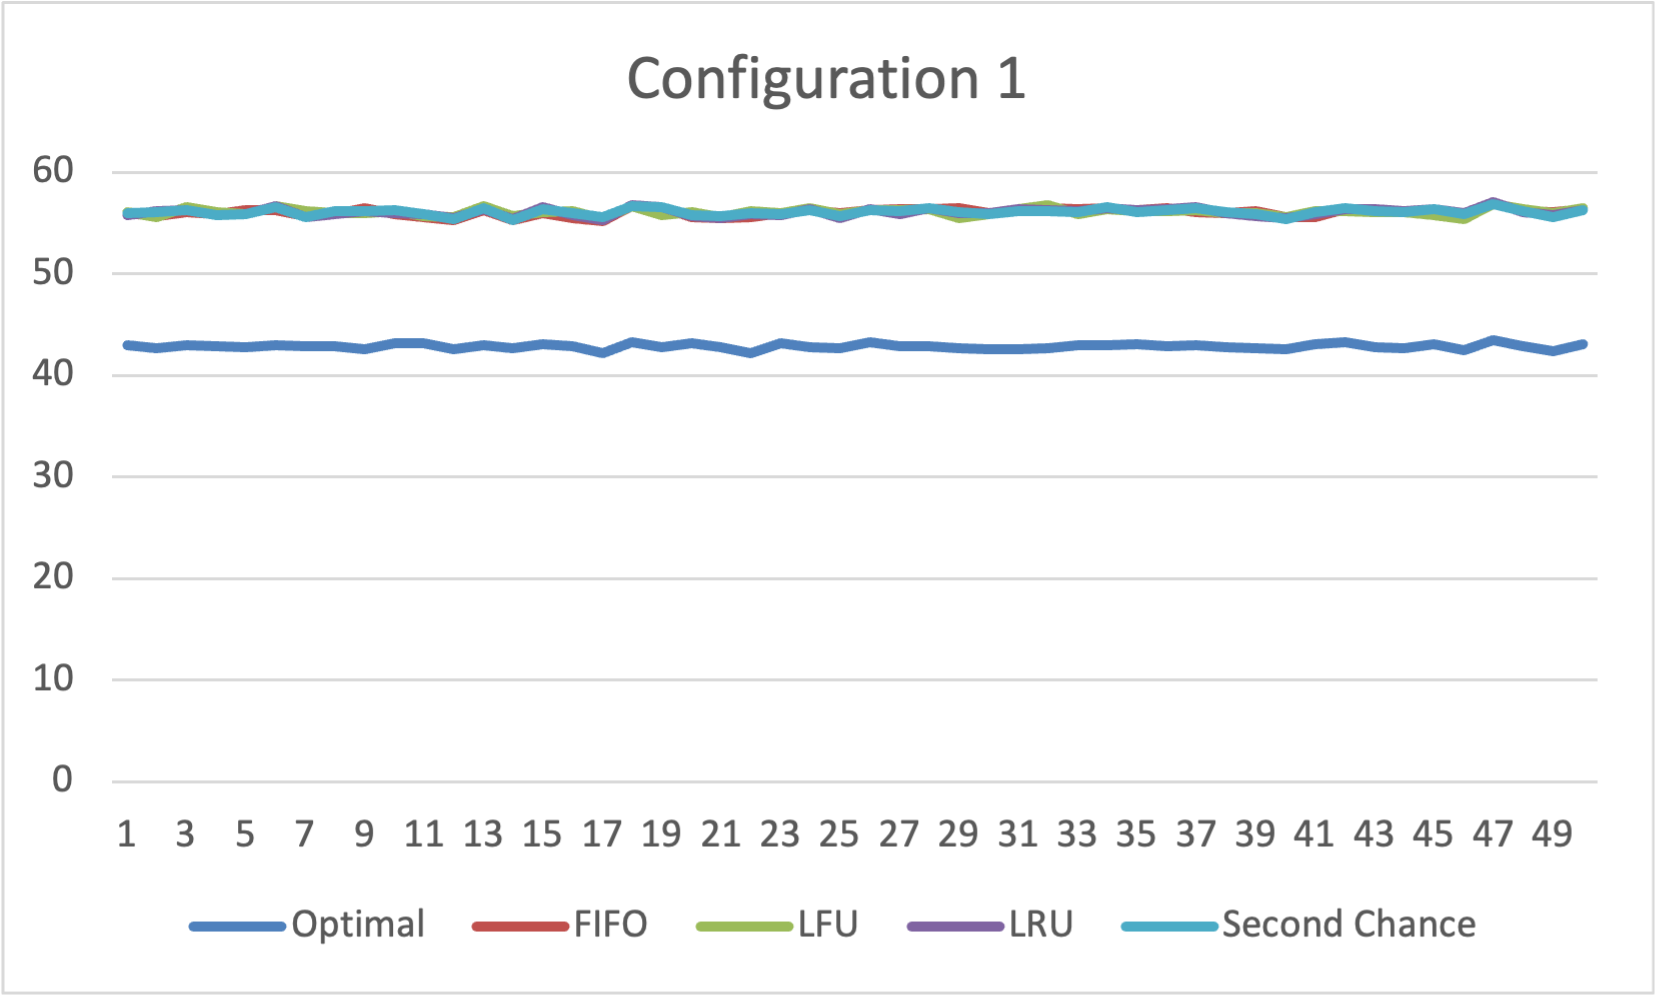
\includegraphics[width=0.5\paperwidth]{Configuration1}}
\end{center}

The obvious consistency states that for the usecase of small devices that count into the section of 
ubiquitous computing with limited functionality there is definetly a need for more efficient paging algorithms. The tracking difference
between optimal algorithm and the other algorithms are significant. All current algorithms are very similar in performance. Therefore, there is 
a very high need for this field of applications. \\ \\

\underline{2. Low memory; long reference; low page variety} \\
\begin{center}
    \makebox[0.5\textwidth]{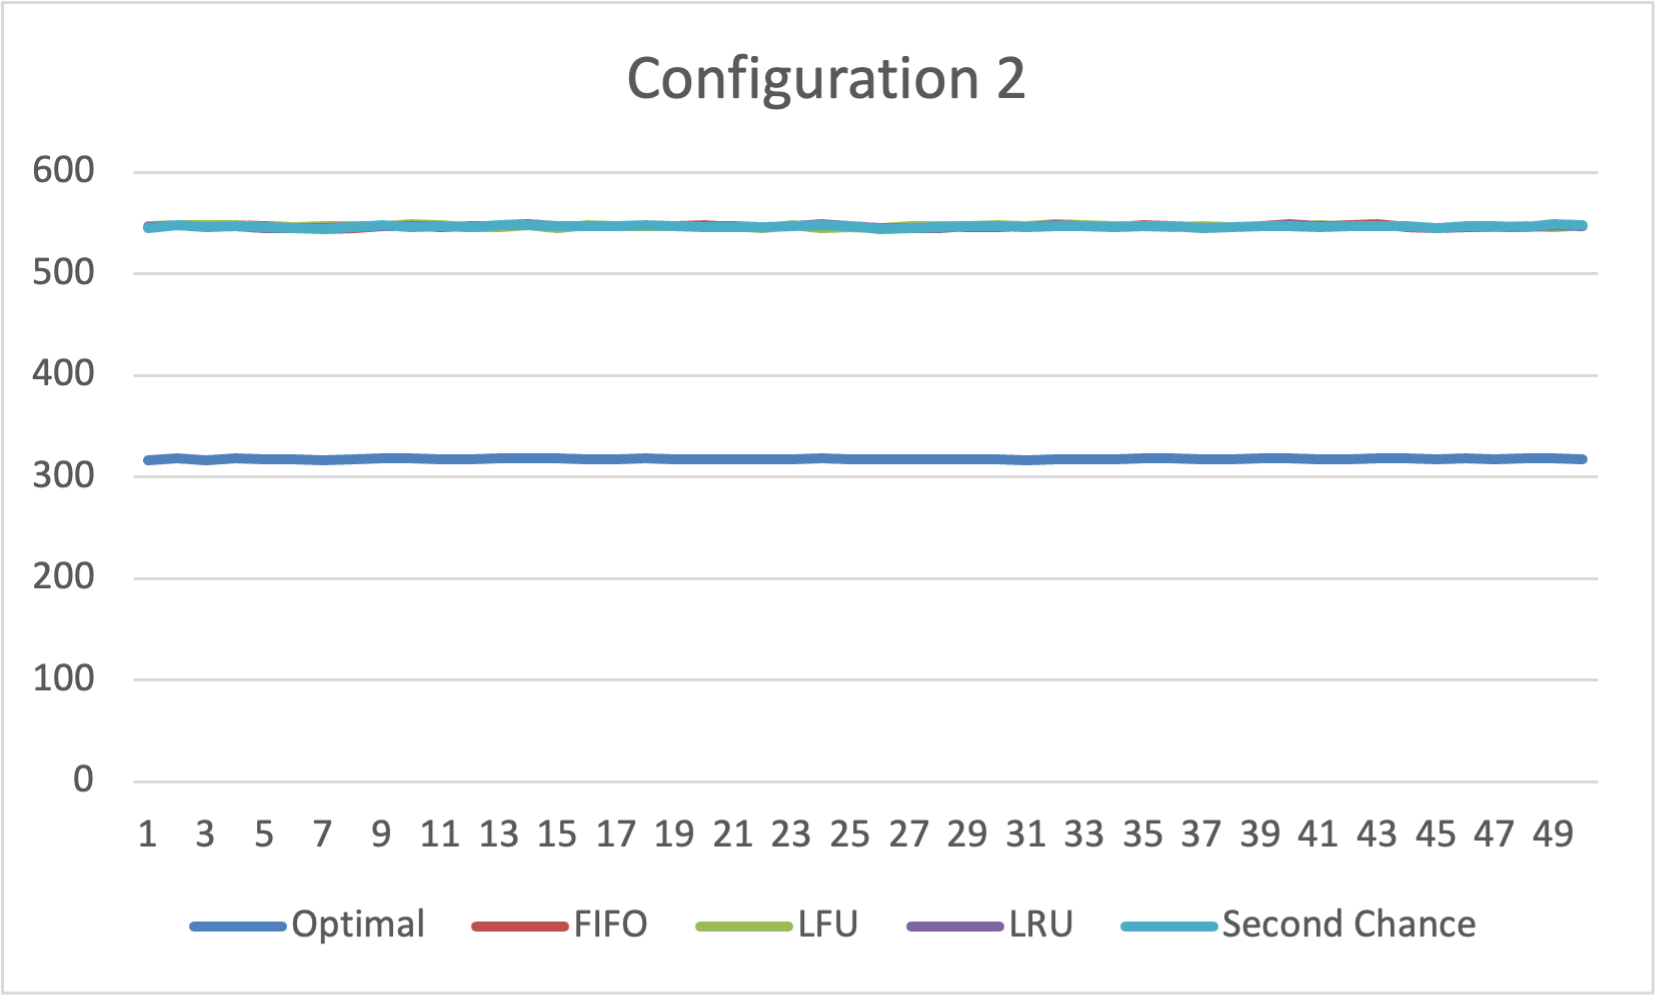
\includegraphics[width=0.5\paperwidth]{Configuration2}}
\end{center}

The tracking differnence of this simulation is proportional to the the difference of the first simulation. This can be interpreted as the fact that
the length of the memory reference does not matter. The only impact of the low memory with a long reference is the performance due to the large amount
of page replacements. The need of a new paging algorithm that comes closer to the results of the optimal one is eqivalent to the need of the first simulation. 
Therefore, it is definetly required to find a more efficent algorithm. \\ \\

\underline{3. High memory; short reference; low page variety} \\
\begin{center}
    \makebox[0.5\textwidth]{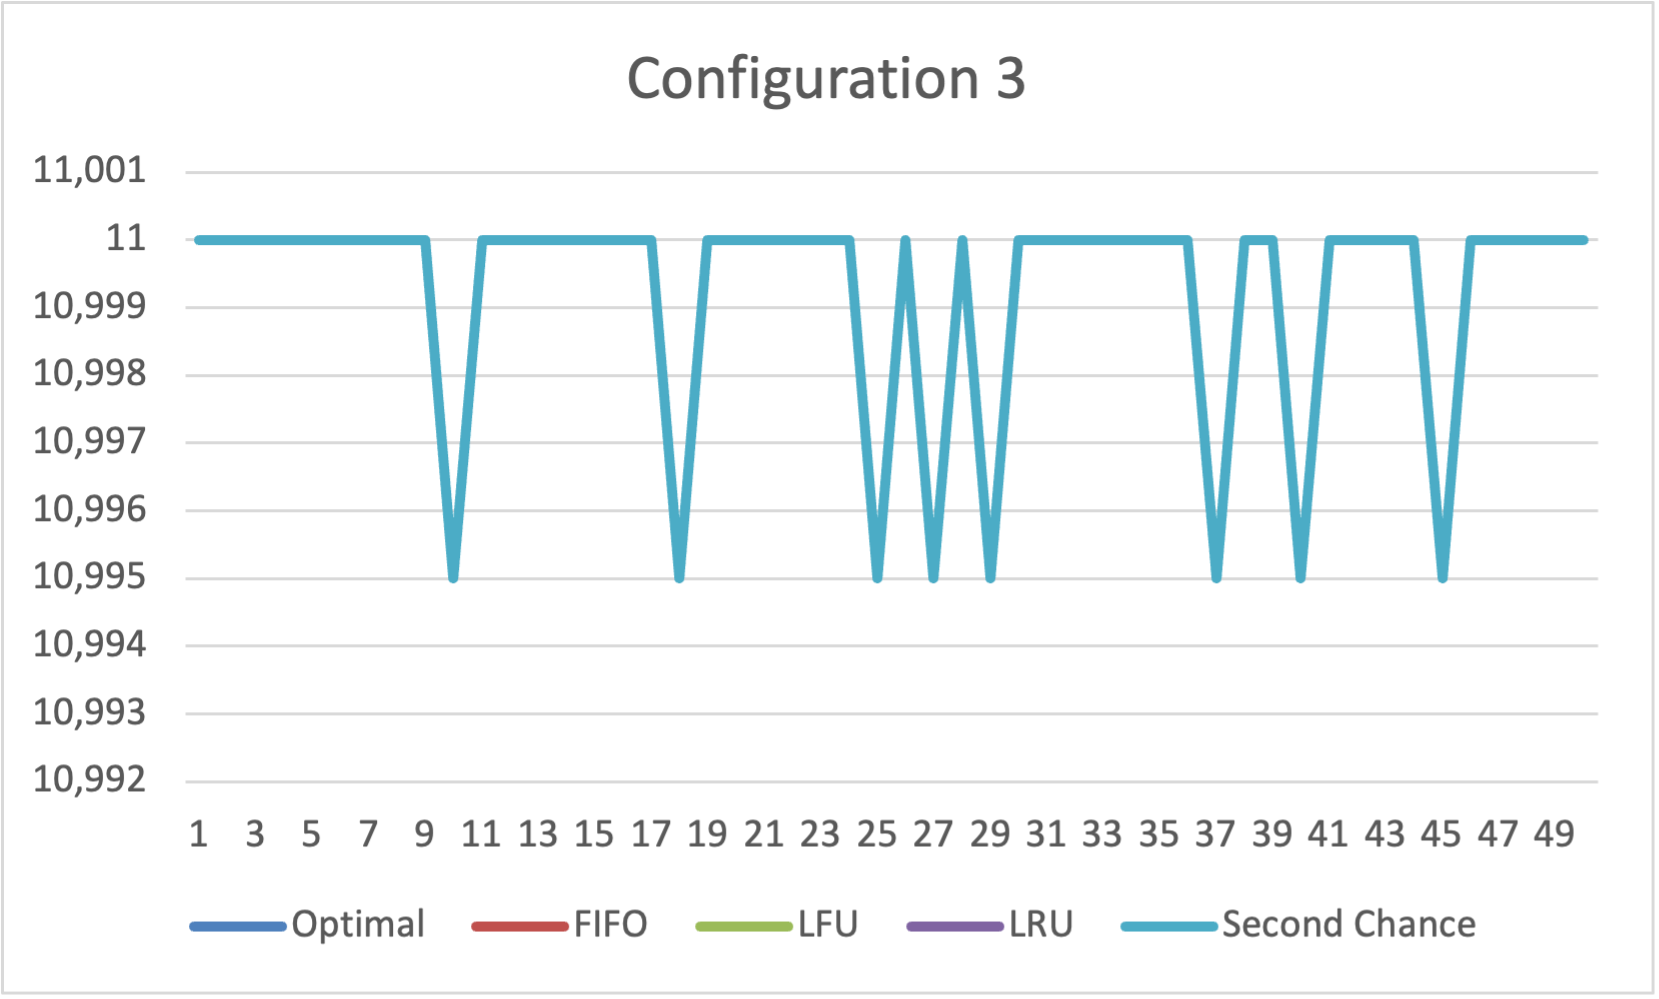
\includegraphics[width=0.5\paperwidth]{Configuration3}}
\end{center}

From this values you can definetly extract that for this specific usecase there is no need for a new paging algorithm. Due to the high memory available 
there are not many page faults are happening which leads to equal efficiency of all algorithms. These types of devices are pretty rare which means these results 
may not be as respresentive as others. \\ \\

\underline{4. High memory; long reference; low page variety} \\
\begin{center}
    \makebox[0.5\textwidth]{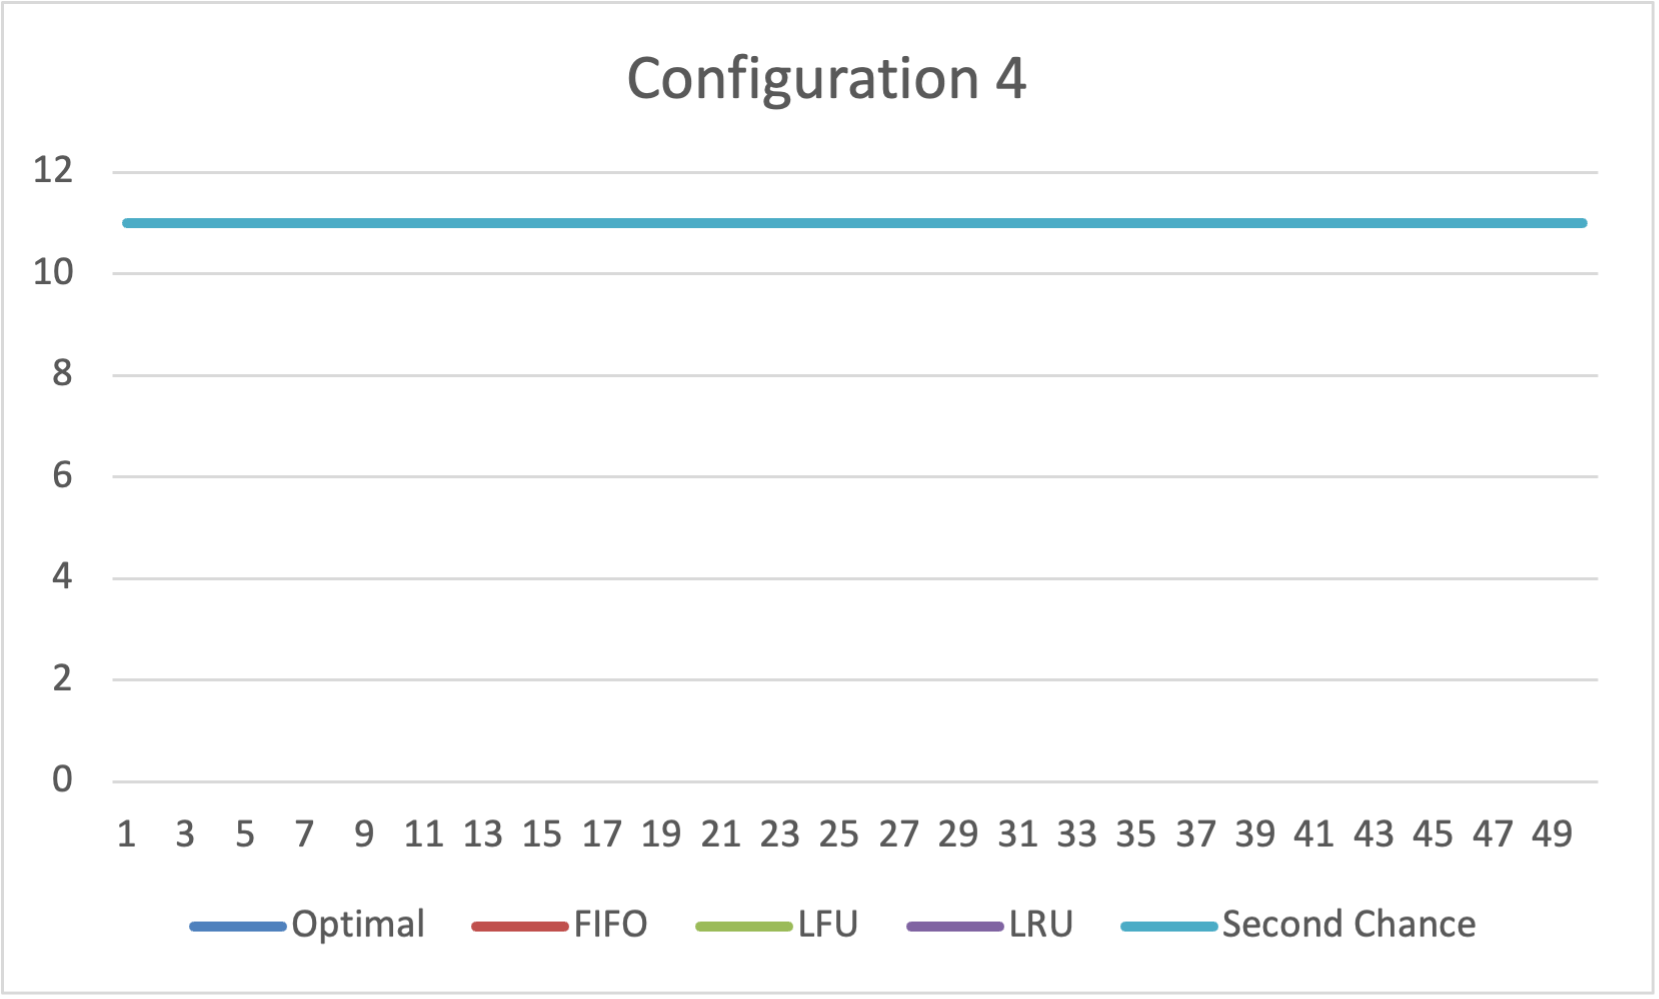
\includegraphics[width=0.5\paperwidth]{Configuration4}}
\end{center}

The results are similar to the results of the third usecase. This can be explained with the low page variety. It leads to a very small amount 
of page faults which means the tracking difference between the algorithms is close to zero. In this case the length of the reference does not have any effects 
on the results, because the pages are already stored in memory. Therefore there is also no new paging algorithm needed for simple desktop applications. \\ \\

\underline{5. Low memory; short reference; high page variety} \\
\begin{center}
    \makebox[0.5\textwidth]{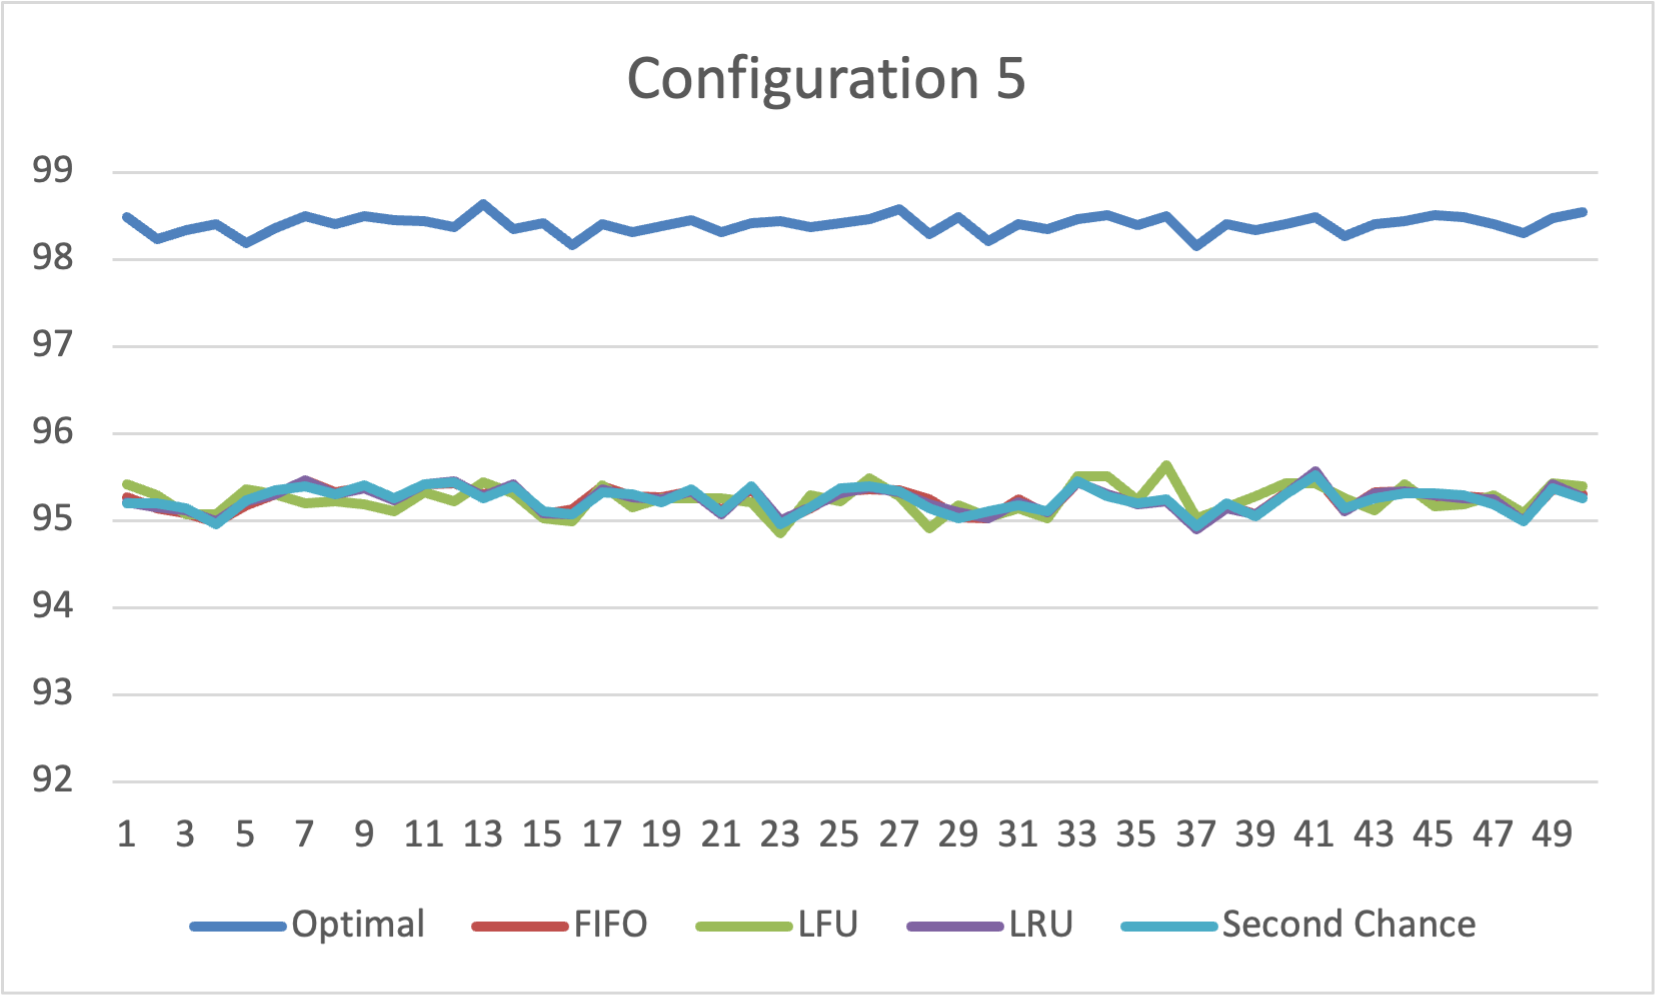
\includegraphics[width=0.5\paperwidth]{Configuration5}}
\end{center}

Thiese results firstly may seem strange, but can be ecxplained easily. Due to the short reference there are not many page faults happening, even if the 
page variety is high. This scenario is very interesting for future applications and shows that for this type of small devices there is definetly no need for more 
efficient algorthms. Moreover, there might be more of a need of an adjusted optimal algorithm that can handle short references more efficient. But it can be possible that
there will come other load allocations for this devices. This is a non predictable scenario due to the improvements and developments going on in the area of ubuquitous computing. Therefore,
I would say here might also be a need for more efficient algorithms in future, if you take current trends into consideration. \\ \\

\underline{6. Low memory; long reference; high page variety} \\
\begin{center}
    \makebox[0.5\textwidth]{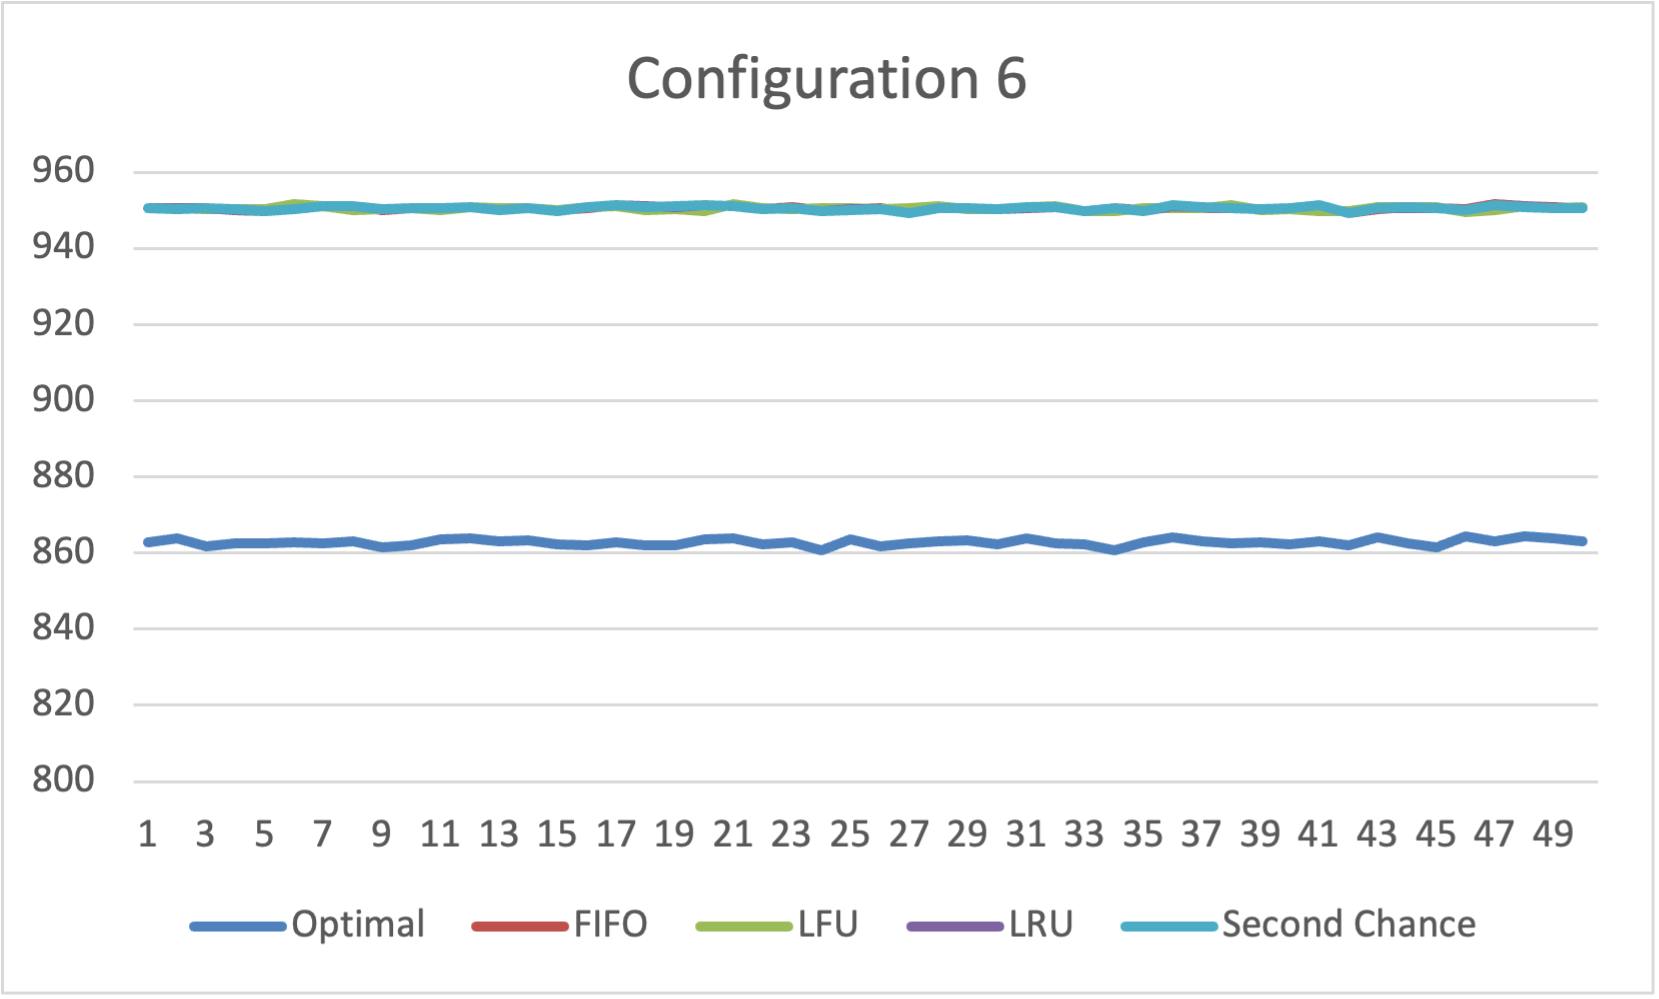
\includegraphics[width=0.5\paperwidth]{Configuration6}}
\end{center}

With a long reference the results are much clearer in comparison to scenario 5. Long references are leading to an increasing amount of page replacements which
leads to an larger tracking difference. If we also take current IoT trends into consideration it is crystal clear that we will need better replacement algorithms, 
because the amount of data to process is increasing more rapidly than the performance if we talk about Moores law. \\ \\

\underline{7. High memory; short reference; high page variety} \\
\begin{center}
    \makebox[0.5\textwidth]{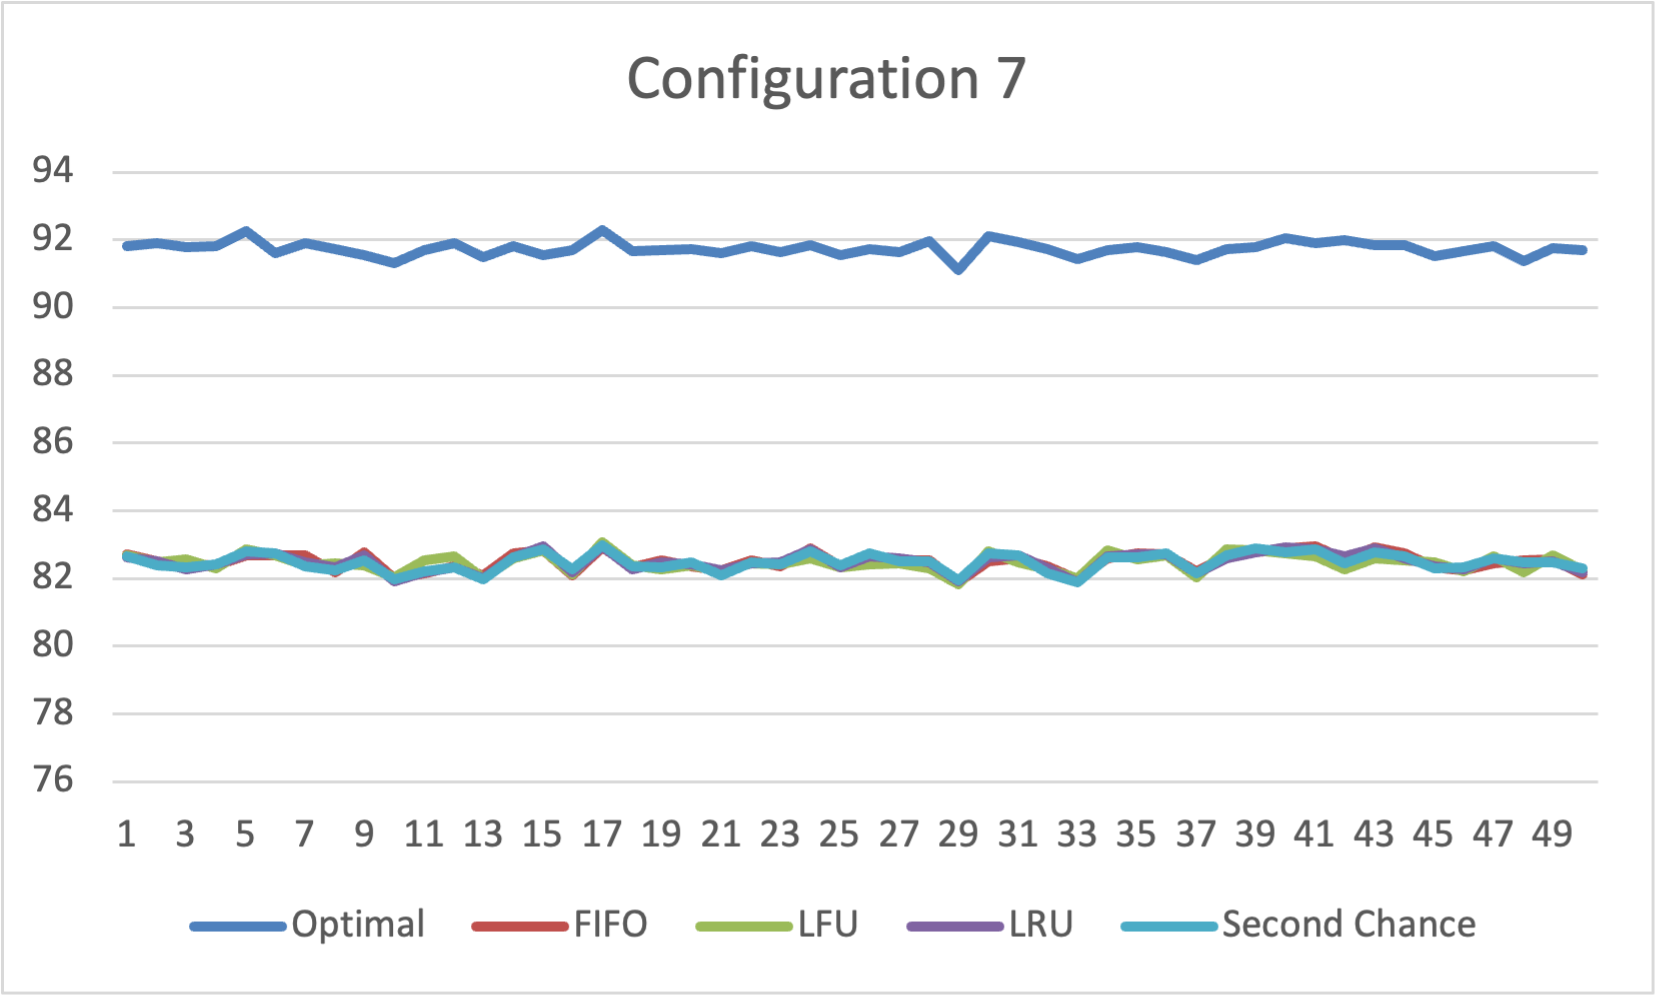
\includegraphics[width=0.5\paperwidth]{Configuration7}}
\end{center}

If we talk about high response time devices we also may think that there would be a need for better algorithms. But if we take a look at the reference
length of a typical application in this field, we clearly can see, that the need of more intelligent page replacements are not given. It might be even easier to increase
the page size to make access to memory easier for these types of applications. Moreover, increasing memory size to an economically acceptable value 
might also be cheaper. \\ \\

\underline{8. High memory; long reference; high page variety} \\
\begin{center}
    \makebox[0.5\textwidth]{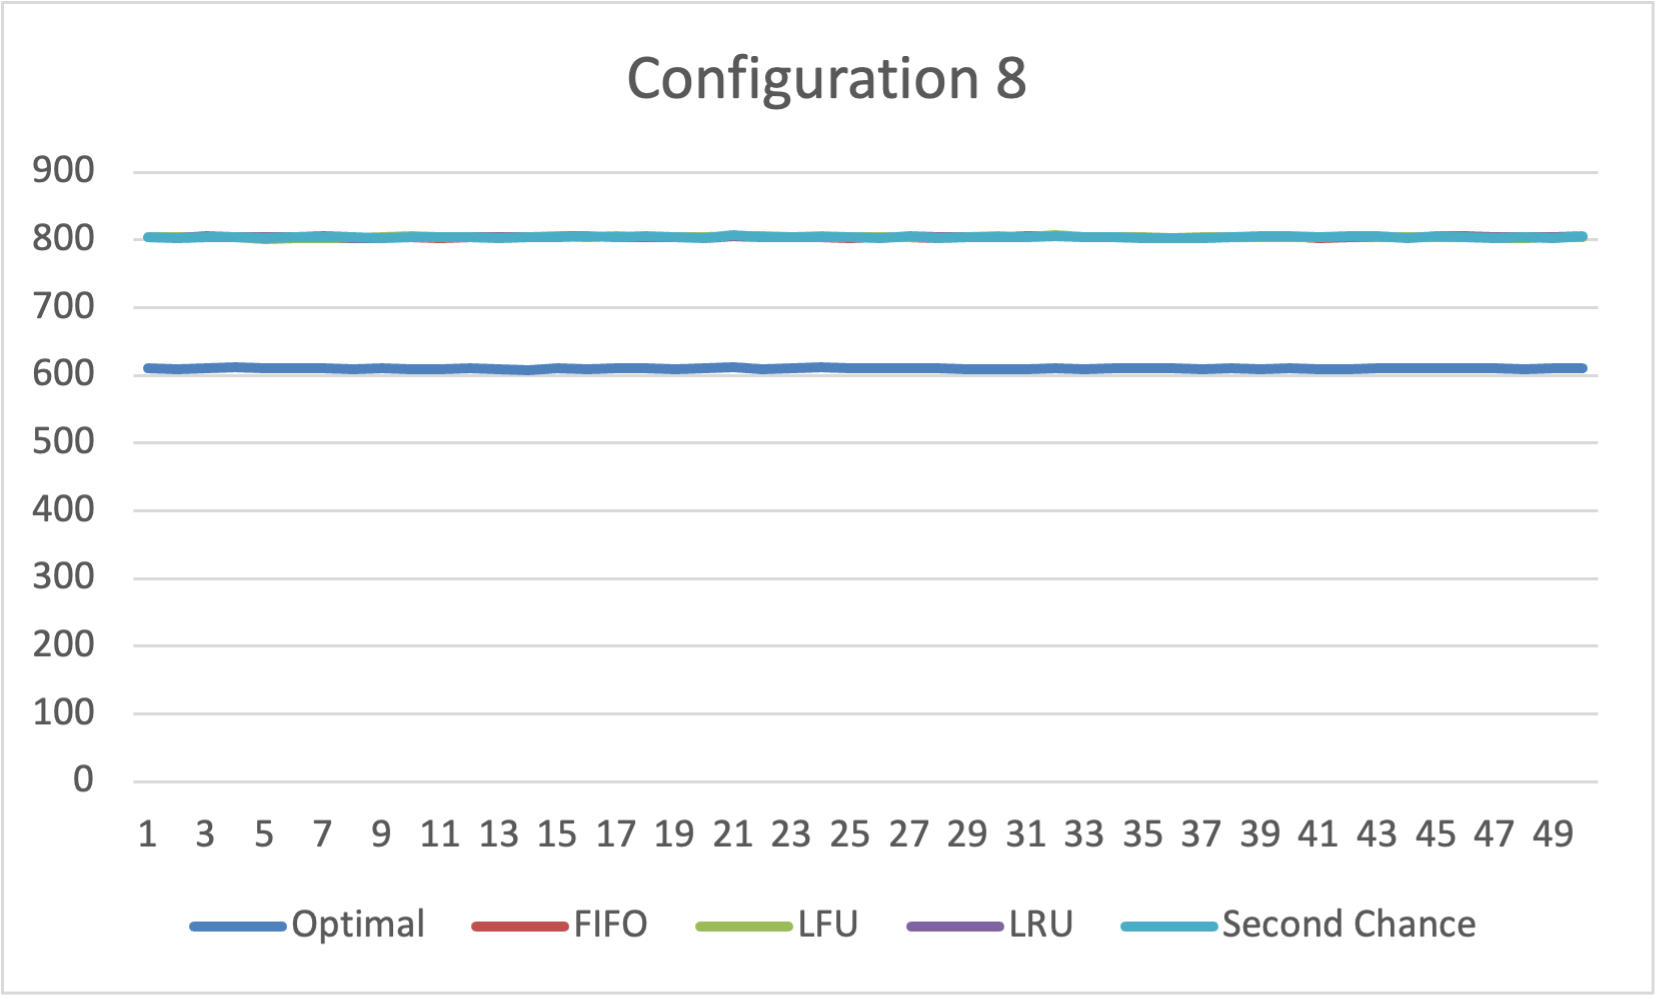
\includegraphics[width=0.5\paperwidth]{Configuration8}}
\end{center}

The tracking difference of the optimal algorithm to the other algorithms is quite large. This means there is a big need for more efficient algorithms. 
Large amounts of data are a real problem of the future and the present. Therefore, with higher amounts of data and longer references there will be always a need
for new paging algorithms, because increasing the memory size is less cost efficient.

\section{Interpretations}

If you sum up all results of all different scenarios, it seems crystal clear that we need more efficent paging algorithms for all possible applications in the future and in the present.
Cost efficiency is much higher, because increasing memory sizes will cost forever and science only once. \\
Because of the missing depth of results it cannot be clearly interpreted how fast a new algorithm should be to fit future applications. To make a
safe prediction we need to take also other factors into condieration. An two dimensional graph does not have to ability to predict future scenarios with clearance. \\
There is also the question about priotized algorithms within of complex multitasking environments of future computing environments. Modern operating systems are usually handing page replacements
within their process scheduling. This means only the current process is allowed to replace memory pages. The priority of memory replacements so depends on the priority of scheduling algorithms.

\section{What about prioritized algorithms}
We earlier talked about the possibility and probability of priotized page replacement algorithms. In future environments there might also be real process multitasking, which means 
the scheduler can apply two processes at the same time. Therefore, both processes run with different priorities. This leads to the question if we will need prioritized algorithms for paging applications. \\
The question if quite simple to answer: Yes. But this also means that the results of this research only fit to single scheduling environments. Therefore, it is hard to say if these results may
apply to future applications. In present we can say that we will need better algorithms but not about the future. But we can start a thought experiment. Currently the priority of paging algorithms is given by the priority of the parent process
scheduling algorithm. This means that the process scheduling algorithm has many child memory managment (paging) algorithms. These algorithms are dependent on each other on both sides. \\ \\

Now lets imagine a mathmatic function that tries to bring all these memory management algorithms together. Every process has its own area of memory in which it operates. This means every algorithm is continuous in a specific area of memory. As a descriptive function it would look like this: \\
\begin{math}
    f_{n} \colon D &\to B,&\quad f_{n}(x),&\quad D = [x_{n0}, x_{n1}]
\end{math}

If we want to combine this function into one single function that is equal to the scheduling function we will get something like this:\\
\begin{math}
    t(x) = 
    \begin{cases}
        f_{0}(x), &\quad x \in [x_{0},x_{1}) \\
        f_{1}(x), &\quad x \in [x_{1},x_{2})\\
        f_{2}(x), &\quad x \in [x_{2},x_{3})\\
        f_{3}(x), &\quad x \in [x_{3},x_{4})\\
        \text{...} \\
      \end{cases}
\end{math}

For clearance the sum of the range of each interval would be the total amount of memory: 

\begin{math}
    \text{Memory size} = \lim \limits_{n \to \infty} \sum_{n=0}^{\infty} |f_{n}(x_{n}) - f_{n}(x_{n+1})|
\end{math}\\
\begin{math}
    \lim \limits_{n \to \infty} \int_{0}^{n} t(x) dx = \lim \limits_{n \to \infty} \sum_{n=0}^{\infty} |f_{n}(x_{n}) - f_{n}(x_{n+1})|
\end{math}

Because every memory management algorithms operates with its own memory allocation table, which are physically continuous, we can state:
\begin{math}
    \lim \limits_{x \uparrow x_{n}} f_{n}(x) = \lim \limits_{x \downarrow x_{n}} f_{n+1}(x)
\end{math} \\

Therefore, we can say that $t(x)$ is continuous and therefore it is possible to design a memory management algorithm that contains priority and is 
on the same abstraction layer as the process scheduling algorithm. This means, we can only have one memory management algorithm and one process scheduling algorithm for any amount of processes. 
This means future multi process scheduling scenarios are not at all scary for modern computer science. We are able to design such algorithms.

\section{Conclusion}

To put it in a nutshell, there is definetly a need for better scheduling algorithms in the present and future. Even if some edge cases may exist in which the current algorithms are efficient enough or even faster than the optimal (unadjusted). 
The important usecases are predominant which means it is economically useful to search for new algorithms. Even in possible environments with real multitasking (multiple seperate process scheduler)
we can develop new algorithms that are based on single threaded scheduling. We do not need to worry about possible multitasking environments, because they can be adopted easily. Developing algorithms therefore should be considered everywhere.
We also need to take private institutions like tech firms into condieration, because they will have the most economic advantages. So including them into current research may improve the 
process a lot. As a final short answer I would call the need for new page replacement algorithms enormous. 

\section{Further information}

This paper is not officially published by any university or HAW. It is private research that is not proven yet by any certified academic institute. Therefore, it cannot be used 
as a prooven starting point of research or as proof for a theorem. It can just be used as a starting point of further academic research with the restriction of proving this paper first.


\end{document}